\documentclass{mproj}
\usepackage{graphicx}
\graphicspath{ {./images/} }

\usepackage{fancyvrb}
\usepackage[final]{pdfpages}
\usepackage{times}

\usepackage[newfloat]{minted}
\setminted[python]{fontsize=\footnotesize}


\usepackage{tcolorbox}
\usepackage{caption}
\usepackage{subcaption}

\BeforeBeginEnvironment{minted}{\begin{tcolorbox}[colframe=white!25!white]}%
\AfterEndEnvironment{minted}{\end{tcolorbox}}%

\newenvironment{code}{\captionsetup{type=listing}}{}
\SetupFloatingEnvironment{listing}{name=Code Snippet}


\begin{document}

%%%%%%%%%%%%%%%%%%%%%%%%%%%%%%%%%%%%%%%%%%%%%%%%%%%%%%%%%%%%%%%%%%%
\title{Source Control Integrated Issue Tracking - The Next Generation of Issue Tracking}
\author{Nystrom Johann Edwards}
\date{7th September, 2018}
\maketitle
%%%%%%%%%%%%%%%%%%%%%%%%%%%%%%%%%%%%%%%%%%%%%%%%%%%%%%%%%%%%%%%%%%%

%%%%%%%%%%%%%%%%%%%%%%%%%%%%%%%%%%%%%%%%%%%%%%%%%%%%%%%%%%%%%%%%%%%
\begin{abstract}
Two software engineering tools are mainly used for collaboration during software development. They are issue tracking systems (ITS) and version control systems (VCS). Maintaining both systems is cumbersome and can reduce productivity if the focus is continuously switched from developing code to maintaining issues. The combined system provides a reduction of the friction between both activities. It shows that the next generation of issue trackers can utilise the power of VCS allowing developers to embed and maintain issues directly in source code. The combined benefit provides an accurate description of the state of any software project by providing one source of truth. Using a novel solution, the Source Control Integrated Issue Tracking (SCIIT) system aims to eliminate the friction by extending the VCS to manage issues embedded within the source code. Developers can now update issue information, track development progress, manage collaboration, and inspect complex relationships between their issues and source code as issues are attached to version controlled commits.

Keywords: Issue Tracking, Version Control System, Embedded Issues, Source Code, Git
\end{abstract}

\pagenumbering{roman}
\educationalconsent
\newpage

\section*{Acknowledgements}

I would like to thank my supervisor, Dr Timothy Storer for exposing me to new software engineering possibilities through this project, for his advice and mentoring on creating a new and useful software tool, and most importantly for assistance in making the difficult decisions on design choices.

I would like to thank my wife Virginia for her support and encouragement throughout my programme and all her efforts to ensure that it was completed with great success. I would not have gotten this far without her support, her motivational speeches and her uplifting presence.

I am especially grateful to my sister Zophia who has financed my programme and has always believed in supported and encouraged my software development talent. She will always be one of my greatest supporters.

I am grateful to my mother Joslyn and all other members of my family that have invested in my education and encouraged me in this undertaking. Their efforts will always be greatly appreciated.

Finally, I would like to thank my colleagues at the university that helped in the evaluation of the project that provided the feedback needed to make a good solution.

%%%%%%%%%%%%%%%%%%%%%%%%%%%%%%%%%%%%%%%%%%%%%%%%%%%%%%%%%%%%%%%%%%%
\tableofcontents




%%%%%%%%%%%%%%%%%%%%%%%%%%%%%%%%%%%%%%%%%%%%%%%%%%%%%%%%%%%%%%%%%%%
\chapter{Introduction}\label{intro}

\pagenumbering{arabic}
\section{Background}

Issue Tracking Systems (ITS) are at the forefront of collaboration tools for software development. Developers track issues as a means to build up information on development tasks. Issues are development tasks including work to create new features, fix bugs, prepare for releases, refactor old code, or any other such task. When developers work on the task or issue progress made it is recorded in the ITS which provides vital information to managers and the team.

Version Control Systems (VCS) are also collaborative. However, at their core, VCS systems are about tracking the progress of the development history of source code for the software product. The product’s source code is managed in a VCS repository as a series of changes called commits. The VCS controls the entire collection of commits for a repository, allowing changes to be created, restored, revised, branched or merged. Developers create commits in a VCS repository that represents progress made on the code and functionality of the software product.

The two systems are used in the development process. The VCS is related to the product as a working growing artefact and the ITS is related to planning tasks and maintaining knowledge on segments of the software product. During development, however, priority is placed on commits to the VCS repository since it is a significant part of daily activities and a representation of an evolving software product. Work on ITS is viewed as a non-priority task and usually falls behind code development.



\section{The Problem}

The friction between the development activities comes from the fact that maintaining the issue tracker lags behind developing code. Developing and delivering code is a priority in order to meet customer deadlines and thus issue tracking work can be neglected. The planning and monitoring of software development activities, however, indicates software project health. As such, and in modern software projects, the ITS is the core system for managing healthy projects. Eliminating or reducing the friction between maintaining the issue tracker and developiing code can therefore lead to better software project health and a higher quality software product.



\section{Objectives}

The objective of this project is to reduce the friction between maintaining the issue tracker and developing code by creating a new system that integrates both activities. Objectives of the system are as follows:

\begin{enumerate}
  \item To embed issue information into the source code of software products.
  \item To track issues along with code commits made to a VCS repository.
  \item To use commit information of the VCS repository to inform on issue progress.
  \item To provide a lightweight alternative to traditional ITS.
\end{enumerate}


\section{Contribution}

This project introduces a new system to reduce the friction between maintaining an issue tracker and developing code. The Source Control Integrate Issue Tracker (SCIIT) System created is a novel system that embeds an ITS into a VCS. Issues are embedded into the source code of a software product and tracked alongside commits in a VCS repository. It thereby allows developers to remain collaborative on issues and productive on writing code into version control. Evaluation of SCIIT shows that it impacts both software development and issue tracking. It can potentially create a new paradigm for the way developers manage and create software.


\section{Structure}

This report is organised in the following structure:
\begin{itemize}
  \item Chapter 1 introduces the problem of friction between maintaining an issue tracker and developing code.
  \item Chapter 2 discusses literatue and related products that are relevant designing a new system to adressing the problem.
  \item Chapter 3 illustrates how such a system is designed and what considerations are necessary for success.
  \item Chapter 4 outlines steps taken in its implementation of mechanisms in order to achieve a robust solution.
  \item Chapter 5 evaluates the solution for correctness, accuracy, usability and its impact on software development activities.
  \item Chapter 6 concludes with future work recommended to improve the system.
\end{itemize}


%%%%%%%%%%%%%%%%%%%%%%%%%%%%%%%%%%%%%%%%%%%%%%%%%%%%%%%%%%%%%%%%%%%
\chapter{Analysis}\label{analysis}

This section analyses the problem in more detail by discussion of the literature to support the need for developing a system that maintains the current value of an ITS. It also looks at current products and how they are used to address the problem and concludes by discussing the key concerns that the solution must address.


\section{Literature Survey}  

An outline of the history of Issue Tracking Systems shows why they are relevant to software development. Throughout history, development teams rely on systems for storing and cataloguing development work. Many systems exist that support software project management but ITS evolved from Bug Tracking Systems which manages information developers utilise to solve errors during software maintenance.

According to Delugach \cite{Delugach:2007}, bug tracking is based on process models for bug reporting, monitoring and resolution. These systems require several pieces of information on the category, description, steps to reproduce, and effect of bugs on software. They also require development teams to assign persons for triage, to update the status, and to comment on steps taken to resolve the issue. Delugach shows processes of Bugzilla and Trac that are quite cumbersome. They include many steps and move the problem through various status levels which requires developers to input information at each stage. Developers, however, prefer simple processes to get the job done.

In their research, Fan et al. \cite{Fan:2017} assert that these complicated processes models for bug reporting are reduced during the rise of open source projects and the introduction of GitHub. In this era, bugs are rebranded as issues to be solved by the large-scale collaboration of developers. They denote issues as a lightweight method for providing information on a problem. They are also used as a way to request new features. Issues simply contain a title, a text description and a label. This paradigm shift allows for a more straightforward process to manage development work.

ITS continually evolved and are now extensively used not only for maintenance but also the active development of software products. Organisations use ITS to record many different tasks during development. In fact, Bertram et al. \cite{Bertram:2010} states that they are a general knowledge repository of all development tasks and all project stakeholders use the system for determining the health of the project.

These stakeholders include developers, managers, end users, production staff and others that steer the success of the software project. Bertram et al. \cite{Bertram:2010} assert that these stakeholders utilize the information stored in the ITS to create reports, gain knowledge, assess progress, assign priority and other software project management activity. This signifies that information stored in ITS is critical to software success.

Developers are not the only persons responsible for submitting information into the ITS. They are, however, the prime consumers of this information as it details the work required to develop or repair code. This information can often be incomplete, leading to frustrations in defining what work needs to be done. In a survey of 20 Mozilla developers using Bugzilla, Baysal et al. \cite{Baysal:2013} discovered that the primary challenge that caused these burdens is ”Situational Awareness” of issues.

In general, developers try to stay focused on the task at hand. Work tasks identified in the ITS grow quite large, and awareness of the next steps, progress to date, and the status of issues are sometimes lost. Additionally, reporting progress in ITS while writing code is increasingly viewed as a burden. Customer deadlines for delivering functionality take priority and as such vital issue activity information is lost or provided later than required. This is compounded by shifts in development priorities as required by customers. At these events issue progress and awareness are easily lost.

Baysal et al. \cite{Baysal:2013} concluded in their research that there was a need for ITS to be able to provide a developer-centric focus which would help to alliviate this problem. Their  idea runs parallel to Zimmermann et al. \cite{Zimmermann:2009} proposal that in order to improve ITS, the tool must meet developers needs by offering up information that is relevant to their current work and encourages them to maintain issue progress.

Many researchers have looked into improving ITS to support the needs of developers. Some have succeeded in creating such systems or tools. Correa and Sureka’s \cite{Correa:2013} tool integrates issues with StackOverflow to provide better leads to problem-solving. This provides developers with the knowledge they need to implement solutions and be more productive. Kshirsagar and Chandre \cite{Kshirsagar:2015} create middleware for ITS that detects and reduces duplicate issues. Additionally, for similar issues, this middleware also automatically assigns them to developers that have worked on similar past issues. These contributions are successful implementations that are developer-centric.

Undoubtedly, these contributions are considered valuable. However, their use is not commonplace in the software development arena. Additionally, the friction of maintaining two systems still exists as they still require developers to explicitly input issue information and continually check on issue status. The development of code and the maintenance of issues are still tasks that occur in two different systems with different purposes.

Even as ITS improved over the years, other paradigm shifts place burden on the software development process. Another such area is Global Software Development (GSD) where there is intense research. Researchers in this area look into the qualities of software products and processes that are affected by globally distributed development teams. Collaboration and communication which is essential in the planning and execution of any project are massively affected by GSD.

Begel and Nagappan \cite{Begel:2008}, outlines the major problems of GSD which are ”inadequate communication, knowledge management, and project process management.” The coordination of work is difficult to maintain for global teams, and as such, they turn to the use of non-traditional methods to achieve their goals or they tend to abstain. These alternatives are mostly chaotic approaches and cause difficulties in software project management.

Fauzi et al. \cite{Fauzi:2010} postulate that in GSD, developers at one site become unaware of the work that is taking place on other sites. This leads to delays in making modifications to the software products as they do not have the information from other sites to make informed decisions. They also allude to the fact that there are no formal processes to address ”lack of coordination and group awareness.” These combined problems can lead to a breakdown of control over software project management.

In order to engage developers in the process, integrated tools are needed to encourage increased collaboration and communication. These tools allow the development process to become simpler as a part of the developer's daily routine. Version Control Systems (VCS) and the source core repositories they manage is one such tool. VCS manage the source code artefacts produced by developers and keeps a history of the changes that were made to the codebase over time. This allows global teams to work on one codebase which allows all those are collaborating on the code to see the entire scope of development.

VCS provides a robust framework for developing code. Prior technologies such as Subversion relied on a centralised structure for version control. In a client-server model, code would be checked in and out of the server but check in processes had high potential to create problems. Git made the process easier by allowing branching code and merging branches to be a more straightforward and quicker process to resolve.

Bertino \cite{Bertino:2012} illustrates by research that Git has significant performance gains over other types of VCS. It allows developers to possess a local copy of the full codebase which makes merging code safer and more efficient. Bertino also shows that the ability to ignore binary and other generated files result in smaller repositories. These files can be compiled from the mission-critical code which is stored in the VCS. This creates for a much more efficient development ecosystem where problems arising from buggy development code can be easily reverted. Developers can work in their own self-contained branches until the code has been tested. These and many other advantages made Git a prime target for widely successful open source projects with many globally distributed collaborating developers.

In a related study, Brindescu et al. \cite{Brindescu:2014} investigate the impact of Git on developer activities. They show that developers are more comfortable creating branches and independantly developing code than they would if they needed check out from a slow centralised system. The improvements allow for the rapid development of features, quick introduction of patch fixes and mass contribution from developers. The authors also make several behavioural observations that all point to developers contributing frequent small commits, working on series of commits in a branch that is related to issues referenced by an ITS, and providing higher quality commit changes.

Even as VCS have evolved to prodive better workflows and processes for the development of code, ITS as existing an a separate environment have not provided comparable workflows to allow for better eficiency. This still does not change the fact that both are critical tools in the software process and both require active attention to be useful. Developers, however, spend most of their time focusing on developing code using VCS as producing code is the ultimate goal of in the process to deliver products to the customer. All other tasks run parallel to supporting this goal.

For the development of the next generation of issue trackers, Just et al. \cite{Just:2008} illustrate that successful products will address ”the quality of information in issues, communication between developers, reduction of work for developers, and automation.” Embedding the ITS into VCS provides four capabilities to address modern approaches to ITS in GSD environments listed below:

\begin{enumerate}
  \item It will be a robust way of building up a knowledge base. 
  \item It will provide a secure method for storing changes over time.
  \item It will encourage collaboration and communication in a global/distributed teams.
  \item iIt will remain the central focus of developers.
\end{enumerate}

By embedding overlapping traits of the ITS with VCS, developers can uniquely utilise an integrated system that meets the needs of both maintaining issue tracking information and developing code.


\section{Related Products}

There are many products on the market that integrate aspects of the ITS with the VCS. Research suggests that those products, while able to draw reference from the VCS, are not designed as an integrated product. While, there are many related commercial products, this report focuses on GitLab, Redmine, JIRA and Fossil as examples. It looks at Bugs Everywhere as an open source project example.

\subsection{Commercial Products}

GitLab, Redmine and JIRA all provide users with some integration with its ITS. Using hashtag references within commit messages, developers can mention work done on an issue. This method is cumbersome as it forces developers to remember issue ID numbers and does not eliminate or reduce the need for them to access the ITS to view changes to the issue description, comments and discussions on the issue itself.

Fossil is marketed as a Distributed VCS with an integrated bug tracker. The entire product is indeed only one executable binary. The bug tracker, however, is a centralised SQLite database of immutable issues, accessed and managed through a local web interface, launched as a command line option of the binary. The ITS also linked using hashtag references in commit messages.

\subsection{Open Source Products}

Bugs Everywhere, as an open source projects, is described as a distributed ITS working along with any choice of distrubued VCS. Although development on the product has ceased since 2013, contributors have been able to create distributed issues. However, they are not attached to commits, they are attached to branch references, and are managed separately from the ITS. An issue is represented as a unique object with a reference to a repository branch. Comments on the issue are also unique objects and are referenced to the issue. These issues are also not embedded into the VCS repository but stored the similar manner and structure as distributed VCS. A command line utility is used to manage the ITS. It still does not do a sufficient job at reducing friction.

\section{Key Concerns}

Based on the problems outlined in literature and the shortcomings of related products, this project intends to address the key concerns regarding reducing friction between issue tracking and developing code while maintaining the collaborative quality of issue trackers. The following is a list of concerns:

\begin{enumerate}
  \item The embedded ITS must do as little as possible to distract the developer from creating code. Valuable information about the development of an issue must be automated and drawn from the commits in the VCS.
  \item The embedded ITS must be able to allow developers to collaborate on issues within a distributed environment.
  \item The embedded ITS must not impede the benefits of the VCS which are to allow developers to easily branch, merge and contribute to the code.
  \item The embedded ITS must not impact on the functionality of the VCS and as such the VCS should be able to operate without the embedded ITS.
  \item The embedded ITS must provide situational awareness on the progress made on issues. These include the branches in which issues exist, the participants in issue development, the detailed log of issue work completed, the changes to issue details over time and the status of the issue.
  \item Issues in the ITS must be related to segments of code where the work must be implemented. This provides the developer with a level of focus on what must be done within that file or piece of source code.
\end{enumerate}



%%%%%%%%%%%%%%%%%%%%%%%%%%%%%%%%%%%%%%%%%%%%%%%%%%%%%%%%%%%%%%%%%%%
%%%%%%%%%%%%%%%%%%%%%%%%%%%%%%%%%%%%%%%%%%%%%%%%%%%%%%%%%%%%%%%%%%%
%%%%%%%%%%%%%%%%%%%%%%%%%%%%%%%%%%%%%%%%%%%%%%%%%%%%%%%%%%%%%%%%%%%
\chapter{Design}\label{design}

This chapter discusses the two main categories of design decisions necessary to embed an ITS into a VCS. Firstly, is the choice of VCS which is critical for the success of the integration and must contain options allowing it to be extended and manipulated. Secondly, is the design for embedding an ITS that give the ability to leverage the versioning functions of the VCS. Next, the chapter discusses the resulting distributed ITS which differs from traditional centralised design. Then it ends with a layout of the software architecture.

\section{The Git Version Control System}

For this project, it is necessary to pick a VCS that is easily extended. Git, the open source VCS, is used as the backbone of the new system. As the most popular open source VCS technology to date, it offers the opportunity to attain vast amounts of information on its internal mechanisms in order to extend it to include custom functionalities such as an ITS. The documentation of Git and the wide variety of related products, articles and examples gives insight into how it is extended. A discussion on its revision control architecture sheds insight on what can be manipulated.


\subsection{Git's Version Control Architecture}

Git’s architecture as described in Gregory's article \cite{BehindGit}, is primarily based on a series of references or pointers to objects which are updated when new changes to files are checked in to the VCS. In Git, each revision of a group of files is called a commit. In each commit, files are stored as a compressed version of the entire file contents (called blobs) and maintaina folder structure by trees. When new commits (additions, modification and deletions) are found, Git, saves the compressed blobs to its objects directory and creates a new reference by hashing the blob’s contents. These references are known as SHA references.

To keep track of the blobs, Git assigns references of them to trees which represent either the folder containing the blob or the root folder of the entire project. The root project folder tree is then in turn referenced to the commit. This way every commit represents the full state of the software project during development. The series of references from blobs to trees and trees to commits are the central mechanism for identifying revisions to files. To determine the files that are changed, it is now just a matter of comparing new hashes of file contents to the corresponding older references.

Since the architecture is based on the assigning and changing of references or pointers, an ITS can be embedded into VCS by assigning references and pointers to objects containing issue information. This way each commit will reference a group of issues. The next section discusses how this can be achieved and how to embed the information in the source code.


\section{Integrating an Issue Tracker System}

\subsection{Embedding Issues into Source Code}

After understanding the architecture of Git, the next step of integration is to find a way to store issues alongside commits. This is achieved by embedding the issue and its related information into the source code of the software project files as a block comment. The only mandatory requirement for embedding an issue is to provide an issue ID using an \textbf{\textit{@issue}} flag. All other information is optional and can be supplied in later commits. Code Snippet \ref{snip:embedded-issue} shows the format of an issue with all optional information in a python code block.

\begin{code}
\captionof{listing}{Example of an embedded issue in python}
\label{snip:embedded-issue}
\begin{minted}{python}
"""
    @issue signin
    @title Create a signin page
    @description
      Create a signin page for users of the website. 
      Include social signin and terms and conditions acceptance.
    @assigned to nystrome, kevin, daniels
    @due date 12 Oct 2018
    @label design, ui
    @weight 6
    @priority high    
"""
\end{minted}
\end{code}




\subsection{Issue Repository and References}

Issues embedded into source code can now be extracted into each local copy of a repository. To achieve this, SCIIT follows the same principle of using references for issues as Git does for commit objects. However, references are assigned to issue objects differently. When a commit is created, the system reads the changes to the source code in that commit and identifies the existence of embedded issues. The contents or information of the embedded issue is extracted and used to form its SHA reference. All the issues identified are then cached to a separate issue repository on the file system for quicker access.

All issue references that are identified belonging to that commit are then collectively assigned to an issue tree. Unlike Git, SCIIT contains just one issue tree per commit. This keeps the SCIIT disk space usage on the file system as small as possible since the creation of may file objects adds disk space overheads. Consequently, any commits that do not contain issues point to the same empty issue tree object. Finally, any issues that is not changed over time is continually referenced on to the next commit.

Each individual issue tree reference is then referenced to a unique object called an issue commit. For all intents and purposes, they contain the reference to a Git commit and a reference to an issue tree. This way they represent the embedding of the ITS into the VCS creating one system that manages both activities.


\subsection{The Integrated System}

As a result of the previous designs, a Source Control Integrated Issue Tracking (SCIIT) System can now be adequately used to represent the complex relationships between the management of issues and the state of the software project. Figure \ref{fig:sciit-filesystem} shows how SCIIT embeds the ITS into the Git VCS on the file system as a series of references when commits are created. Green arrows represent revised or new objects tracked by the system. Black arrows represent unchanged objects that are referenced in following commits.

%update sciit file system image to show sciit is a strong link of commit and issue commit

\begin{figure}[h!]
\caption{SCIIT ITS embedded into Git VCS Filesystem}
\label{fig:sciit-filesystem}
\centering
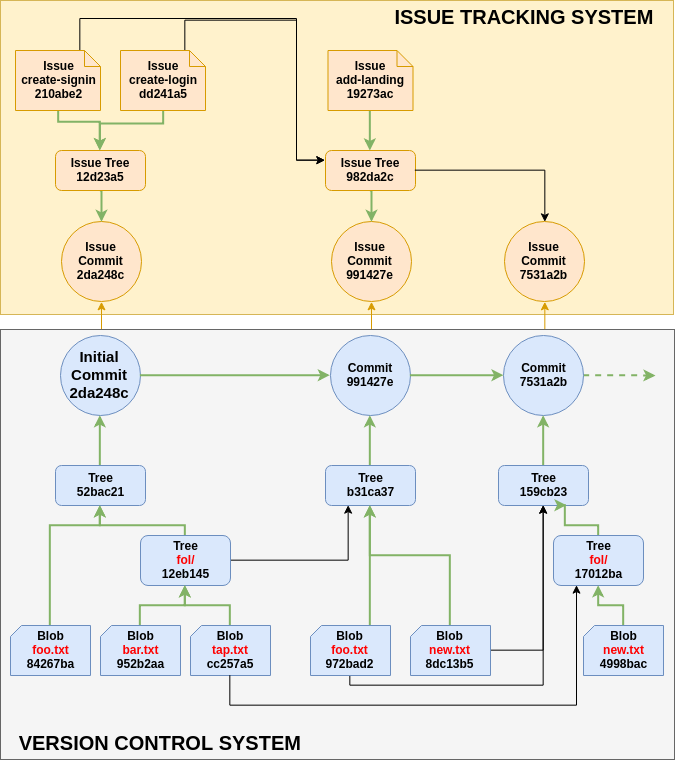
\includegraphics[width=12cm]{sciit-filesystem}
\end{figure}

Figure \ref{fig:sciit-filesystem} shows that every commit made in Git generates an issue commit that contains references to all the changes made to those issues. This, therefore, will pose a change in the traditional management of issues as a commit must be created in order to record a change to an issue. If an issue is changed by editing the issue data embedded in the source code as a comment then a new issue object is created and assigned to a new issue tree when a commit is created. 

Changes to the references of an issue object over time can now be associated with a change in the issue. This is a factor that is taken into account when building the issue tracker history. The issue tracker also intuitively determines if issues are closed by removing references to an issue that has been deleted from the embedded comment. If the issue is no longer in the issue tree at the tip of any Git branch then the issue is closed. This is discussed in futher detail in the next section.

\section{SCIIT's Distributed ITS}

As a result of embedding the ITS into a distributed VCS such as Git, the ITS is also has a distributed structure. In Git, the distributed structure involves the use of branching in which two different series of commits have deviated from one previous commit. Developers can spawn and work in new branches that are parallel to others. When complete they merge their changes with other branches. There are also remote Git repositories on servers where commits on branches are pushed and pulled to and from the local machine.

Although branching and merging, pushing and pulling are the primary mechanisms allowing Git to be distributed, they all are based on the same primitive object, the commit. Since the ITS is based on this primitive object, a branch commit will contain issue commits, issue trees and issues which may change over time. The utility of this design allows for the ITS to also be distributed. The design concept gets compounded in merging scenarios which is discussed in the following example.


\begin{figure}[h!]
\caption{Distributed Issue Tracking in Graph Structure}
\label{fig:distributed-issue-tracking}
\centering
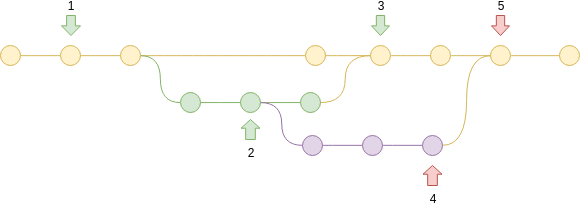
\includegraphics[width=15cm]{distributed-issue-tracking}
\end{figure}

Figure \ref{fig:distributed-issue-tracking} shows a practical example of the distributed ITS embedded into a Git repository branch graph structure. 

At point 1, a new issue is added for the first time into the orange branch. Commits that follow this keep the reference to the issue created here until a user modifies the embedded issue information or removes it from the source code. When branching to green, issue 1 remains open in both branches. At point 2 another issue is created. Here there are two issues open on the green branch and one open on the orange. The purple branch inherits both issues from the green branch. At point 3, developers, for illustration sake, choose to make a simple decision to merge issue 2 into the orange branch. At point 4, both issue 1 and 2 are closed by deleting the embedding from the source code. Here there are no issues on the purple branch. 

At point 5, developers are faced with a decision conflict. They must decide if the work has actually been completed and whether to resolve the merge conflict by deleting the two issue embeddings from the source code, keeping one issue, keeping both issues, editing either or both of the issue information. These decision choices are supported by the Git diff tool which shows the revisions of both the orange and purple branch side by side. The Git diff tool shows the developer the the conflicting areas of the source code where the orange branch contains the embeddings and the purple branch does not. In a distributed team working on this repository, this point gives the team the ability to decide on the final status of the issue. This example illustrates the distributed nature of issues in SCIIT.


\section{Software Architecture}

\begin{figure}[h!]
\caption{SCIIT Software Architecture}
\label{fig:sciit-software-arch}
\centering
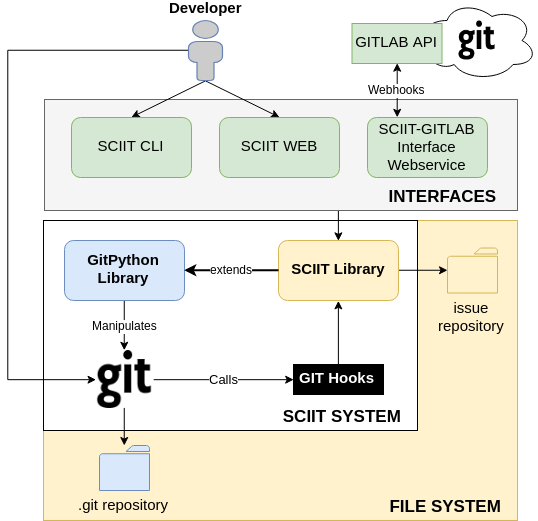
\includegraphics[width=12cm]{sciit-software-arch}
\end{figure}

Figure \ref{fig:sciit-software-arch} shows the software architecture of SCIIT. There is two separate file system storage folders at heart. One responsible solely for the VCS repository objects and the other for the ITS repository objects. The VCS information is accessed by the VCS control tool Git, which in turn can be manipulated by the GitPython Library.

The SCIIT Library has direct access to the ITS repository and is responsible for managing all its objects stored within that context. This is its extended functionality. It also utilises objects, methods, and attributes of the GitPython Library in order to manipulate the VCS repository. With this, the SCIIT Library can use information from both VCS and ITS to create, build and manage issues.

The Git hooks allow for the Git application to call on functions of the SCIIT Library when commit, merge, pull and check out events take place. These hooks allow a level of automation in creating the ITS repository object such that developers need not concern themselves with explicitly maintaining the issue tracker. When these events take place, the ITS is automatically managed.

Interfaces allow users to view issue tracking information stored in SCIIT. They provide direct access to the SCIIT Library that queries the ITS and VCS to build the information needed for the user. All combined these components make up the SCIIT system which allows for the manipulation of VCS and ITS objects.


\section{Summary}

This chapter shows the design of a Source Code Integrated Issue Tracker and how it embeds an ITS into a VCS. The benefit of this allows developers to focus on what they know best which is source code. The next chapter will discuss how these designs were implemented to enable such a system to operate.


%%%%%%%%%%%%%%%%%%%%%%%%%%%%%%%%%%%%%%%%%%%%%%%%%%%%%%%%%%%%%%%%%%%
%%%%%%%%%%%%%%%%%%%%%%%%%%%%%%%%%%%%%%%%%%%%%%%%%%%%%%%%%%%%%%%%%%%
%%%%%%%%%%%%%%%%%%%%%%%%%%%%%%%%%%%%%%%%%%%%%%%%%%%%%%%%%%%%%%%%%%%
\chapter{Implementation}\label{implementation}

This chapter discusses the implementation of the design for providing mechanisms to interact with the integrated ITS. These are the use of Git Hooks for performing issue manipulation at specific Git events; the SCIIT Library which is an extension of the GitPython open source library to manipulate Git objects, Git commands and managing the Issue Repository; and the interfaces required to view and manage ITS information. The chapter shows how issue tracking is performed and concludes with outlining the challenges faced.


\section{Mechanisms}

\subsection{SCIIT Library - GitPython extended}

The first main mechanisms of SCIIT is the SCIIT Library. It is an extension of the GitPython open source library that enables the manipulation of the Git repository with new functionality to manage the Issue Repository. Functionality in the GitPython library that is related directly to the Git repository is extended to provide the extra functionality needed for managing issues. Two programming library objects, in particular, are extended; the ”Repository” object which allows for manipulating the Git repository and the ”BaseObject” object allows for manipulating the raw Git objects (commits, trees, and blobs). Added to these is the ability to manipulate issues, issue trees, issue commits, and the issue repository.

\subsection{Git Hooks}

The second mechanism of SCIIT, Git Hooks, allows for the handling of issues based on Git events. This project utilises three hooks; post-commit, post-merge, and post-checkout. The post-commit hook communicates with the SCIIT library in order to search for embeddings and create issues in the ITS for every commit made. This reduces friction since the programmer does not switch focus to the issue tracker for updating information. The post-merge hook is utilised during two Git events; merging and pulling. In order for SCIIT to be useful to teams, the issues that are created must be syncronised with all members of the team. When pulling commits from the remote repository, SCIIT will build issue objects that are missing. Similarly, during a merge, synchronisation ensures that no issues are missing. The post-checkout hook is similar to the merge in that it syncronises issue with commits. This is mainly implemented for the users that just fetch Git commits from the remote to check out at a later stage.

\subsection{SCIIT Interfaces}

The last mechanism of SCIIT is its interface channels. There are three interface channels that provide three different services.

\begin{figure}
\centering
  \caption{Tracker View in Terminal}
  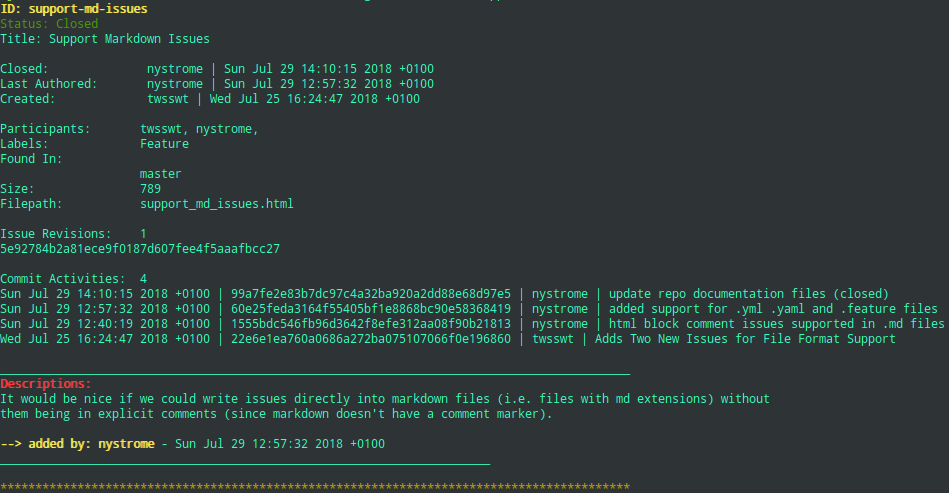
\includegraphics[width=15cm]{sciit-tracker-shot}
  \label{fig:sciit-tracker-shot}
\end{figure}


The first is a command line interface which does not allow for direct manipulation of issues. It allows for users to refresh the issue repository, view individual issues and view the issue tracker. The initialisation command creates the issue repository and builds issues from past commits. This is essential since developers work on existing software projects. They can clone a project and build the ITS by grabbing all the embedded issues from commits. The tracker command allows developers to view details of issues. It shows the complex relationships between the ITS and VCS such as participants, creator, commits to the issue, and changes to the issue over time. This harnesses the power of ITS and VCS such that inference can be made between the two. Further CLI commands and its uses can be found in Appendix B Figure \ref{fig:sciit-cheatsheet}. Figure \ref{fig:sciit-tracker-shot} shows an issue shown at the terminal.

The second is a web interface. This interface shows the issue tracker to the user by launching a local web browser with all the issue tracking information loaded into HTML view. Users are not allowed to edit any of the information within this interface, but it gives a more comfortable display for users to view their issues, read through issue activity and view all other inferred data which performing developing tasks.

The third is an intermediate web service that allows for the integration of GitLab issues with the SCIIT System. The main reason for having such an interface is that it allows for non-developer members of a project such as coaches, team leads, production staff or contributors to create issues in GitLab that will create commits with embedded issues. This module was developed to show that SCIIT and its principles could be integrated with traditional ITS to engage non-developer users. The web service works by using GitLab Webhooks in conjunction with SCIIT on a web server and the GitLab API as follows:

\begin{itemize}
  \item \textbf{Push Webhooks:} These hooks are triggered when developers push commits to the repository. An HTTP request is then sent to the SCIIT web service interface. The interface then fetches the changes from the GitLab remote repository as a mirror repository and syncs the Git commits with the ITS issue references. Any new references that are made by these changes are then packaged, and requests are made to the GitLab Issues API to create or edit those issues. Commit activities related to these changes are added to the GitLab issue as notes.
  \item \textbf{Issue Webhooks:} These hooks are triggered when someone creates or edits an issue in the GitLab web interface. An HTTP request is then sent to the SCIIT web service interface. The interface then takes the issue title and issue description that was changed and makes changes to the relevant source code contents of the file that corresponds to the issue. If it has not been assigned to a file previously a new file is created to track the new issue. It then makes a request to the GitLab Commits API to create a new commit with the specified changes.
\end{itemize}

When this web service is attached to the GitLab remote repository it syncs GitLab issues, SCIIT issues and commits such that the developer need not be concerned that the issues they create or need to work on are not in the SCIIT system. A simple pull from the remote repository will bring in the related commits and refresh the issue tracker and its details. Figure \ref{fig:sciit-gitlab-shot} shows a screenshot of the issues in GitLab managed by the web service.


\begin{figure}[t]
\centering
  \caption{Screenshot of issues managed by the SCIIT web service}
  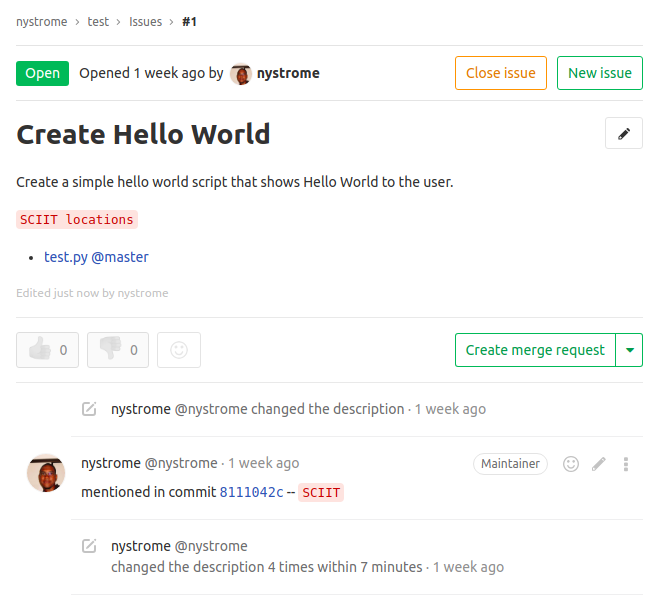
\includegraphics[width=10cm]{sciit-gitlab-shot}
  \label{fig:sciit-gitlab-shot}
\end{figure}



\section{Issue Tracking}

The embedded ITS is no longer similar to the centralised ITS that are commonly found. In fact, the SCIIT Issue Tracker is decentralised and distributed; it is dependent on the graph structure of branches and commits. It is accessed via an interface into the SCIIT Library and is built from a revision of the repository. A revision is a range of commits that are reachable from one commit to another. It can also be specified based on Git’s intermediate references such as the HEAD or branch names and can span a path which may include all commits or those reachable from this branch.

As a distributed ITS, information about the issues are built by traversing the entire repository based on the revision (commit range) specified. Git operations such as the viewing the commit log operate similarly. In this Git operation, commit history inforation is built by traversing the commit graph reference structure like shown in Figure \ref{fig:distributed-issue-tracking}. The commits are scanned and commit information is displayed based on whether the commit is reachable from the revision specified in the graph structure. In SCIIT, to build the issue tracker, commits and issue objects that contain references to each other on this revision path are read, and the complex information between the ITS and the VCS is extracted. The following is a list of such information:

\begin{itemize}
    \item \textbf{Creator:} The creator and the date and time of creation can be identified by the first occurrence of this embedded issue in the commit revision history. The author and time of that commit provide the exact information that reflects the creator of the issue.
    \item \textbf{Last Author:} The last author and the date and time of authoring can be identified as the last occurrence of this embedded issue in the commit revision history. Similarly, this provides the exact information required.
    \item \textbf{Closed:} Again this information is extracted from the last commit mentioned that does not have the embedded issue. The person that has removed the embedded issue is the person that closed the issue.
    \item \textbf{Participants:} This is a list of persons that made commits that contained these issues. It adequately infers who has done work on the issues.
    \item \textbf{Branch Information:} This information is extracted showing the existence of issues on branches, and their status on branches. It can help the ITS user identify where issues are present and the status of their state.
    \item \textbf{Commit Activities:} This is a list that shows the date, commit message and commit author for every commit that has the issue present. It is one of the more powerful influence tools as it can show what work was done on issues over time. This approach has four main advantages.

  \begin{enumerate}
    \item It represents real changes to the functionality and state of the software product as commits are made.
    \item It can contain a commit message the identifies precisely what progress has been made on an issue.
    \item It can tell which developer contributed the change to the issue.
    \item It can give the commit that contains the changes so that it can be reviewed.
  \end{enumerate}

\end{itemize}

The information inferred does not need to be explicitly entered into the issue tracker as it does in traditional ITS. This is the power of SCIIT where users need not be concerned about manually recording such information, but it can be generated for them.


\section{Challenges}

Since the SCIIT system is first of its kind, there are some challenges associated with its design and development. This section outlines the significant design and development challenges.

The first major challenge concerns extracting issues embedded in source code. This involves use of a series of regular expressions. These expressions look at the raw string representation of the source code that is stored in a commit and extracts issue inforation. The first step in the process is to create regular expressions for extracting the block comments based on the programming language of the source file. The second step is to check the block comments for the presence of the \textbf{\textit{@issue}} flag. Once this is found the issue information can be extracted. The regular experssions used for each step of the process is very long and complicated and took some many testing iterations to ensure validity. Many updates to them were made over the development of the project.

The second major challenge concerns the allocation of IDs to the issues in the issue tracker. There were two options. The first option is to allow the system to assign issue IDs to all issues in the tracker once created. This option however was difficult to implement and provided a processing and I/O overhead. The process involved: reading the last generated ID from the disk; incrementing the ID for use in the new issue; saving the new issue to the disk and saving the new issue ID to the disk. These operations are costly in situations where there are many issues to be stored in one commit.

The most appropriate approach to this challenge is to give developer control of the issue IDs to be used. This optimises the disk access during commits and allows for the developers to explicitly specify the issue. A drawback of this approach is the need to check commits for duplicate issue IDs that are sepcified throughout all the source code files of the project. This ensures that there are no two issues in different files with the same issue ID. The system will then warn the user of a conflict of issue IDs and where the conflicts are located.

The third major challenge concerns the single threaded file access operations used in Git. When building the issue repository from past commits or building the issue tracker, SCIIT traverses each commit and scans its related file object contents (blobs) to get issue information. This is a time-consuming process and is restricted to a single thread because of the architecture of Git. SCIIT encounters I/O errors if multiple threads are used since there is a high likelihood that the same file may be accessed at the same time due to the referencing of the issue commit objects to commits. Although the system will benefit from extracting information for two or more commits at a time, I/O operations and access does allow it to be possible. 

\begin{figure}[t]
\centering
  \caption{Screenshot of initialising issue repository from past commits}
  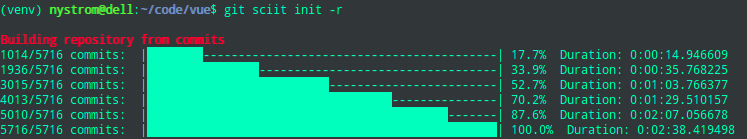
\includegraphics[width=14cm]{sciit-init}
  \label{fig:sciit-init}
\end{figure}

This limits the performance of SCITT to build issues from past commits on repositories that consist of a high number of commits such as the Linux Open Source Project (781,903 commits) or even smaller repoitories such as Tensorflow (39,390 commits). The performance also suffers based on the commit/merge strategy that the developer teams are using since some strategies can have commits that contain a larger tree of file changes that other strategies may not implement. As an average baseline, SCIIT takes 15 seconds to scan 1000 commits. Figure \ref{fig:sciit-init} shows the building of the issue repository from the VueJS git repository containing, at the time of writing, 5716 commits.

This problem also affects the performance of building the issue tracker history as each object must be read in a single thread while traversing the issue commit revisions. For vast repositories, it can take some time for the issue tracker to be built which can reduce the productivity of the developer. One way around this challenge is to provide a revision to the building of the issue tracker that limits the building of the full issue tracker. Here only the information required by the revision is used.

The GitLab integration web service helps to reduce this problem. It does this by storing the issue tracker information between revisions specified by the lastest commit a developer has when pushing to a remote repository and the last commit on the remote repository. In a typical workflow, this is a series of commits that are made on a new branch. The state of the issue tracker between small revisions of commits can now be safely stored in a centralised manner. It must be noted, however, that developer teams may use other remote hosting solutions for which integration services have not yet been created.

The last major challenge concerns the use of GitLab API calls within the web service interface. GitLab Webhooks are a part of the main functionality of the website. For example, utilising the GitLab Commits API triggers a Push Webhook. As such, during development special care needs to be taken to verify the dates of receiving GitLab webhooks with the internal web service time. If a Webhook was triggered and came in within seconds of another, they would be ignored as it would have originated from API calls within the web service. In the web service handling Issue Hooks generated requests for handling Push Hook and vice versa. If this was not carefully handled internally, then the web service would send infinately looping requests, unnecessarily creating GitLab Issues and commits on remote the repository.

\section{Summary}

The implementation of the system ensures that developers are less burdened with the responsibility of maintaining an ITS as all the issues are now embedded into the VCS commits. This should now reduce the friction between maintaining the issue tracker and developing code as the activities are now combined and automated.


%%%%%%%%%%%%%%%%%%%%%%%%%%%%%%%%%%%%%%%%%%%%%%%%%%%%%%%%%%%%%%%%%%%
\chapter{Evaluation}\label{evaluation}

This chapter begins by presenting the evaluation strategy. The remainder outlines user feedback, the impact on issue tracking practices, the impact on developing code using VCS and the robustness of the product as identified through software testing. 

\section{Evaluation Strategy}

SCIIT is evaluated by a process called Dogfooding. In programmer jargon, this is where developers use the product during development to determine useful features to include or to determine fixes to unintended bugs before distribution. It provides high levels of feedback that are rapidly included in future releases. It is worth noting that dogfooding also applied to the development of SCIIT. It is used as the ITS for development work of this project.

Within dogfooding, user testing is conducted for a period of 5 weeks with three students and the supervisor. During this period, users are able to use the software for tracking issues in their own development projects and report feedback. Each tester uses SCIIT in their individual development work and as such user feedback does not include information on team environments. Due to the scope of this project and its impacts on development practices more user and group testing will be required in the future. 

Essential points from feedback are discussed in the user feedback section. The software is also evaluated based on the stated objectives and the benefits and drawbacks of the design of the system.


\section{User Feedback}

This section describes the user experiences when using the SCIIT system. In particular, it will cover feedback on merits and drawbacks relating to the reduction of friction between maintaining issue trackers and developing code, its ease of use, how well it displays issues.


\subsection{Reduction of Friction}

% rephrase this section with comments from sarthak and quy

SCIIT provides a significant contribution to reducing the friction between maintaining issue trackers and developing code. It allows for developers to be able to focus on the task of writing code and creating commits. In the background to this process, SCIIT tracks revisions to issues and its references to commits. This way work can be done on an issue without the need to manually update some ITS.

If the developer wishes to view the status of an issue, they can call on the issue tracker from the command line interface or web interface and view the progress that has been made. Since it is built directly from the references of Git and Issue objects, the developer gets additional information. It is inferred and outlines other developers working on the issue, the issue creator, who closed the issue and what has been done. This information exists in this format for all members of the team without the need for it to be manually or explicitly defined.

When the need to change details of an issue arises, the developer does not need to login to another ITS or move their focus away from the code. The embedded issue can be easily found using a text search in an IDE or through calling the tracker command from the CLI to be directed to the file containing the embedded issue. The developer can then make their updates to the metadata of the issue to include or remove the necessary details.

Additionally, since the issues are stored as embeddings within the source code, a clone of the repository will give a full copy of the issue history. This works well for new developers joining the team and does not require team leaders to set up two accounts for access to the codebase and access to issues. The issues are self-contained within the code of the relevant project. This quality can also be useful in open source projects where the issues can be transferred during project forks. Finally, it saves the space and infrastructure required to maintain traditional ITS.

By maintaining issues in this manner, the system shows that a significant step has been taken to reduce the friction between the two development activities of maintaining the ITS and VCS. The developer now needs only concern themselves with pulling and pushing code to the repository where the issue tracker will seamlessly build, track and maintain issues in the background.

This does not mean that developers are not responsible for looking at the embedded issues and performing the work required to implement them. However, it allows them to work in an environment with one point of contact. The design of SCIIT allows for developers to trod along writing code and to care for the issue tracking process. Additionally, the issue tracker will now be up to date with the state of each revision of the source code.

\subsection{Ease of Use}

Test users find the application easy to install and use. They note the ease of creating and managing issues by embedding the information into the source code. The status messages shown after commits on the command line are useful for them to maintain awareness and confirm the status of issues at each commit. This is provided by the Git Hooks. They noticed that they did not need to expressly comment on each activity as the commit messages were used.

\subsection{Interfaces for Viewing Issues}

As for interfaces, most users found that the web interface provided by the application was very basic in providing information. The web interface was simple enough to use, but it did not provide them with the quality that they were accustomed to. They stated however that the command line interface was straightforward to use and liked the fact that the tracker command had three different detail levels. This way they were able to decide on what level of detail was required when viewing the issues.

\subsection{Benefits and Drawbacks}

The most commented on drawback is the local web interface. Many users would have liked more control over the issues at this point to be able to edit descriptions and other metadata. Since the issues are embedded into source code, it was difficult to provide this function. Another stated drawback was the need to have comments on an issue.

The most highlighted benefit was the capability of continuing developing code while issue information is built up over commits. They found that they did not need to remember issue numbers as this was internally tracked. They also liked the fact that they could embed and move the issue to segments of code where the development work is taking place. They mentioned it as helpful in providing a quick glance on what needed to be done without leaving the code editor.



\section{Impact on Issue Tracking Practices}

This section discusses the impact of SCIIT as a new paradigm of existing technology. SCIIT proposes some radical changes to the methods in which issue tracking is currently performed. In a traditional sense, ITS is meant to be a centralised system containing all the knowledge objects in essentially one database. Considering the distributed environment and that work is done in Git on branches, it could be challenging to capture all the information for all issues on all branches without conflicting data.

Fortunately, Git also allows for the querying of revisions such that all commits on all branches are returned maintaining their parental links. This allows us to keep the valuable issue data for each project in a suitable archive. There is a limit to this however and circumstances where there is a potential for the loss of valuable data.

The product currently has no protection over the deletion of Git references. Indeed this is handled by Git itself which allows users to delete branches and to use functions such as rebasing that allows the manipulation of commits and references. In cases such as these the issue commits may lose their references and there is a potential to lose those issues and its data forever, however few it may be. A permanent store may be required for the issues at some points of the development process to prevent such events.

Use of the integration web services such as the provided GitLab web service can provide a solution. Information from the intermediate references between issues and commits are permanently stored in GitLab when a developer pushes to the remote repository. Additional to this, the web service also allows for non-developers to interact with the SCIIT system where issues created in a traditional ITS creates commits with embedded issues in the VCS. This allows for developers to remain focused on creating code while not shutting out other organisational users of the ITS.

The integration of the traditional and SCIIT ITS provides just a method for more collaboration between various types of organisational users. This is an interim approach to maintaining the levels of collaboration in the development of software. As SCIIT matures, it can influence both the development of ITS and VCS such that interim services are no longer required.

\section{Impact on Developing Code Using VCS}

This section discusses the impact that SCIIT can have on developing code using VCS since it is the backbone component of the system. There are three development practices in VCS that are impacted by the integration of an ITS; pulling commits from remote collaboration repositories, creating detailed commit messages, influencing development workflows and branching strategy.

The integration of issues and code encourages developers to pull often so that they can have the latest changes made by other team members. Pulling often allows for the VCS and the ITS to be updated with the latest information. This is currently a software development best practice, as developers working in teams may contribute changes that affect the work of others. This form of collaboration and communication keeps the developer teams aware of other work processes that are required to create high-quality software products.

Commit messages in SCIIT are used as the basis for the log of work done on an issue. This encourages the use of detailed commit messages stating what has been changed added or fixed. Additionally, it also gives a higher quality status for the VCS as the messages used will provide a history of precisely what the commit contributed to the software product. Persons collaborating on this repository can now search the commit messages to find information on how to implement particular functionality, information on what was required to fix a bug, or information for educational purposes. This practice facilitates the ability for higher recall from the repository and benefits all members of the team.

Branching strategies are currently used to primarily manage the way in which software is merged. There are many theories for branching strategies, and they help developers to follow a particular workflow when creating code so that their changes can be quickly integrated without significant problems. SCIIT is mainly designed to be useful to feature branching. This is where a developer creates a new branch of code from the main development branch in order to implement a new software feature. When work is done, the feature is merged into the development branch or testing branch for integration testing and validation with the other code of the software product.

In SCIIT feature branching allows users to create their issues at the beginning of that branch and work on that issue till completion. Additionally, any branches from this feature branch can be considered to be related to this issue and also means that work done here contributes to the issue related to that feature. At the conclusion of the feature branch, the issue can be closed and merged. SCIIT’s influence on feature branching allows issues to remain in their own development line and is logically separate from other types of work. This can be seen apparent in Figure \ref{fig:distributed-issue-tracking}.

These areas are potentially affected by SCIIT and are a practical improvement to the workflow of developers. It encourages best practices and workflows that are industry standard. This, however, may not work well for all developer teams as some prefer to adopt their own style of developing. Further use of the product in various different developer environments is required in order to ascertain any broader impact on development and VCS practices that SCIIT may have.


\section{Software Testing} % should I bother having a testing section

This section describes in detail the testing strategy that was used to verify the design and validity of SCIIT. The software is tested after the implementation of each desired feature this allows for regression testing with features already implemented. The test suite also utilises many mocks which mask the dependencies on other code in the system. Each test that requires access to the full Git repository is mocked out such that the test suite would finish running in sufficient time. Lastly, continuous integration (CI) practices are used to run the test suite as regression testing each time code is committed.

All modules of the software, except the integration web service, were thoroughly tested with unit and integration tests at the time of writing. However, the integration web service tests are live to confirm its functionality. The test suite for the application is modular. The SCIIT Library, command line and web interfaces we all tested separately and a TestCase is made for each method within each module. Each TestCase contains atomic tests that verify the functionality of the method by checking valid and invalid scenarios of operation, errors thrown, and boundary conditions. Currently, the test suite consists of 142 tests providing 98\% code coverage and verifies the stability of the application.

During development, CI practices were used to test regression of the application. Regression is where new functionality added breaks with the well-structured behaviour of methods. CI is where the entire test suite is run on every push to the remote repository. GitLab’s CI is used since it offers the ability to send notifications on failed test cases. In these situations, the application can be immediately updated to ensure that functionality is maintained.

This complete testing framework ensures that the SCIIT system developed conforms to the designs set out. This, however, does not mean that SCIIT is entirely free from bugs. More widespread use of the system will uncover more bugs as users may try operations with the system that does not conform with its design intention. However, at its current release, the system is stable for distribution and use.

\section{Summary}

The SCIIT system introduces changes in the way developers conduct software development practices since the ITS is embedded into the VCS. The software practices are an emergent property of this design. Continued use and adoption will inform changes to development workflows as a result, and the system will provide more insight and evaluation over time. However, at this stage, it is thoroughly tested and has a stable release for distribution.


%%%%%%%%%%%%%%%%%%%%%%%%%%%%%%%%%%%%%%%%%%%%%%%%%%%%%%%%%%%%%%%%%%%
\chapter{Conclusion}\label{conclusion}

This project shows that Issue Tracking Systems (ITS) can be successfully embedded into Version Control Systems (VCS) to reduce the friction between maintaining an issue tracker and developing code. The solution is a Source Control Integrated Issue Tracking (SCIIT) system that saves issues alongside commits in Git.

SCIIT benefits developers by allowing them to focus on the development process and create code. Issues are tracked by creating a small embedding in a block comment of the source code which is automatically tracked alongside the commits that developers create containing the issue. Through this, developers are unburdened with the need to explicitly update an ITS.

The system provides a lightweight method for tracking issues and potentially introduces new development workflows. Additionally, the system is a first of its kind and needs to mature before it shows additional benefits or unintended drawbacks from its use. It currently contains a feature set that allows it to replace traditional ITS but future work can be done to include features that enhance team collaboration.

\section{Future Work}

As discussed in the literature, the ITS is a repository of knowledge that drives software development and learning. In order to continue in this vein, SCIIT must include other features that are present in traditional ITS.

Adding the ability to comment on an issue is critical to communication. Comments on issues allow developers and various other stakeholders to discuss the effect of the issue on the software product or enterprise. For example, production and infrastructure teams may comment on an issue to give input on how it would affect the deployment of the software product after development.

Currently, SCIIT has no mechanisms for storing comments on issues. Creating such a mechanism will allow SCIIT to be much more valuable to developer teams and as such, it is the next high priority feature item to be developed into this product. Once it is included, it must again be tested for validity and be evaluated for its contribution to the software development process and its impact on VCS and ITS activities.

Commit activities is another area in which the system can be improved. Currently, commit activity is defined as any commit that contains the issue. This is not entirely accurate as teams may include issues of the software product as a guide of what work must be done. These issues may exist in the system however no work may be done on the issue until the appropriate time.

This leads to the need for context-aware and programming language specific mechanisms that mark when work on an issue is actually started. Context-aware mechanisms can be implemented through a marker on the issue to identify its state such as future work, work in progress, or paused state. This way commit activity can be attributed to the accurate state of an issue which does not depend solely on its existence in the source code.

Programming language-specific mechanisms can also be used to identify when work done on the source code relates to the issue. For example, issues present in a module or function block will have dependencies on other modules or functions. If the source code of the dependency has changed, then SCIIT can identify this as a commit activity on the issue.

These additional features will make the SCIIT system more robust and attune to the needs of both development teams and other software product stakeholders.


\appendix % first appendix
%%%%%%%%%%%%%%%%%%%%%%%%%%%%%%%%%%%%%%%%%%%%%%%%%%%%%%%%%%%%%%%%%%%
\chapter{Command Line Cheatsheet}
\begin{figure}[h!]
\caption{SCIIT Command Line Interface Cheatsheet}
\label{fig:sciit-cheatsheet}
\centering
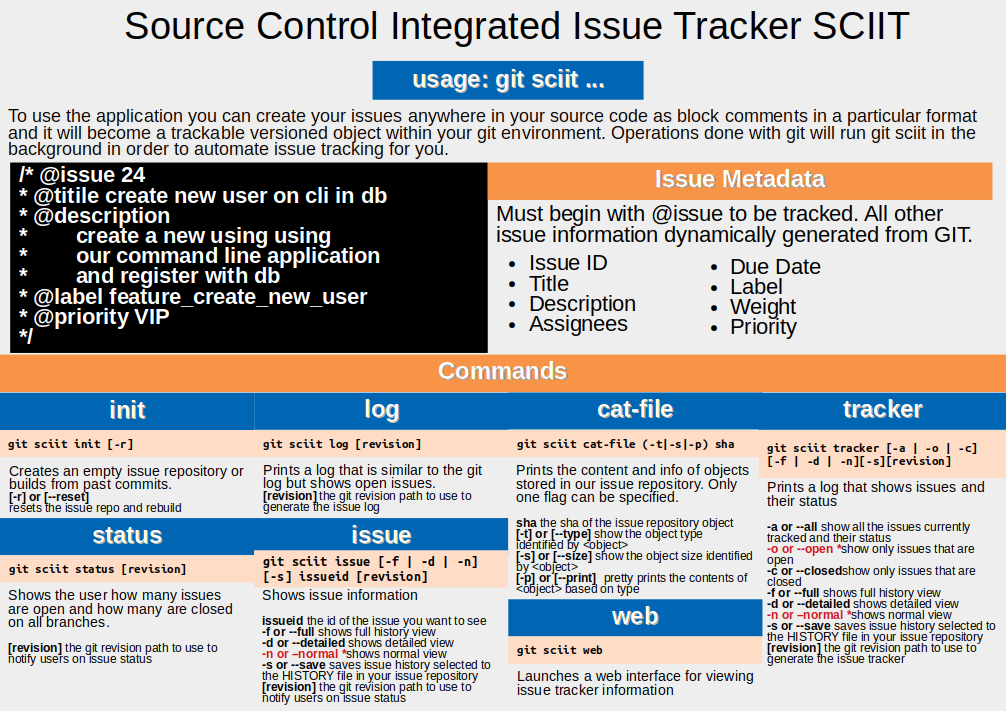
\includegraphics[width=16cm]{Cheatsheet}
\end{figure}

%consider making a diagram for the sciit webservice

%%%%%%%%%%%%%%%%%%%%%%%%%%%%%%%%%%%%%%%%%%%%%%%%%%%%%%%%%%%%%%%%%%%
% it is fine to change the bibliography style if you want
\bibliographystyle{acm}
\bibliography{mproj}
\end{document}
